\documentclass[12pt]{article}
\usepackage[left=2cm, right=2cm, top=2cm]{geometry}
\usepackage[utf8]{inputenc} 
\usepackage{mdframed} %For framing the title
\usepackage{graphicx} % to include images
\usepackage{amsmath} % For math mode
\usepackage{caption} % For captions
\usepackage{subcaption} % To use caption while using mini page
\usepackage{amssymb} % To use math symbols
\usepackage{multirow} %To combine multiple rows in a table
\usepackage[table]{xcolor} %To color rows / columns in table
\usepackage{titling} %To vertically center the title page
\usepackage{hyperref} %for URL

\title{MATH 8650 \\ Advanced Data Structures \\ Fall 2018\\ \quad \\
	Term Project: Week 1 Report \\ Optimization of Bellman Ford Algorithm}
\author{Submitted by: 
\\ Vivek Koodli Udupa 
\\ Sai Harsha Nagabothu}
\date{November - 16, 2018 }

%%To make the title page center vertically centered
%\renewcommand\maketitlehooka{\null\mbox{}\vfill}
%\renewcommand\maketitlehookd{\vfill\null}

\begin{document}
\begin{mdframed}
%Displaying Title
%\begin{titlepage}
\maketitle
%\pagenumbering{gobble}% Remove page numbers (and reset to 1)
%\end{titlepage}
\end{mdframed}
\pagenumbering{arabic}% Arabic page numbers (and reset to 1)

\section{Introduction}
This report addresses the implementation of Naive Bellman-Ford algorithm. The naive version serves as the basis of comparison for other variations of the Path Finding algorithm. \\
\\
The Bellman Ford algorithm returns the shortest path from the source node to other nodes in the given graph. The graph may contain negative weight edges. The algorithm outputs shortest path only if there are no negative weight cycles. Negative weight cycles are reported. \\

\section{Implementation}
The implementation of the algorithm is as follows:
\begin{enumerate}
	%Step 1	
	\item First step is to initialize distance from source node to all other nodes as infinity, and the distance to source node itself as zero. \\
	An array dist[] of size V is created and all its elements are set to "Inf" i.e infinity and dist[source] is set as zero. Here V is the number of vertices in the given graph.
	
	%Step 2
	\item The next step is to calculate the shortest distances. The following steps are repeated V-1 times. \\
	Note: x-y are two vertices and  z is the weight between x-y
	\begin{enumerate}
		\item For each edge x-y:
		\item If dist[y] is not infinity and dist[x] + z $<$ dist[y], then update dist[y]
		\item Updating y, dist[y] = dist[x] + weight of x-y( i.e z )  
	\end{enumerate}
	
	%Step 3
	\item Now check for negative weight cycles. This is done by performing the distance check once more.
	\begin{enumerate}
		\item Do the following for each edge x-y:
		\item if dist[y] $>$ dist[x] + z then report "Negative Cycle".  
	\end{enumerate}
	The idea here is that Step 2 ensures the shortest path if the graph does not contain negative weight cycle. If another iteration through all the edges finds a shorter path, then there exists a negative weight cycle. The algorithm reports this and exits.
\end{enumerate}

\section{Results}
In order to test the Implementation, two graphs were selected. Graph 2 contains a negative cycle. 
\begin{figure}[h]
\centering
	\includegraphics[scale=0.25]{./Figures/w1Graph1.eps} 
	\caption{Graph used to test the BF Algorithm}
	\label{fig:g1}
\end{figure}

\begin{figure}[h]
\centering
	\includegraphics[scale=0.25]{./Figures/w1Graph2.eps} 
	\caption{Graph 2 with highlighted negative weight cycle}
	\label{fig:g2}
\end{figure}

Figure \ref{fig:g1} shows the test set 1 used to find the shortest path. Figure \ref{fig:g2} represents the test set 2 that contains a negative cycle. The algorithm must report a negative cycle for this graph.

\begin{figure}[h!]
\centering
	\includegraphics[scale=0.25]{./Figures/w1Graph1End.eps} 
	\caption{Highlighted Shortest Path for Graph1}
	\label{fig:g3}
\end{figure}

\begin{figure}[t!]
\centering
	\includegraphics[scale=0.70]{./Figures/w1Output1.png} 
	\caption{Output of the algorithm for Graph1}
	\label{fig:g4}
\end{figure}

\begin{figure}[h!]
\centering
	\includegraphics[scale=1]{./Figures/w1Output2.png} 
	\caption{Output of the algorithm for Graph2}
	\label{fig:g5}
\end{figure}

Figure \ref{fig:g3} represents the shortest path found by the implemented Algorithm. \\

Figure \ref{fig:g4} shows the output of the python code for Graph1 and Figure \ref{fig:g5} shows the "Negative Weighed Cycle Present" output for Graph2
\newpage

\section{Next Steps}
For week 2 the following things are planned:
\begin{enumerate}
	\item Modify Bellman Ford to report shortest path even when a negative weight cycle is present
	\item Implement the SPFA ( Shortest Path Faster Algorithm )
\end{enumerate}

\section{Conclusion}
In conclusion, the algorithm calculates the shortest path in bottom-up manner. At first it calculates the shortest distances that has maximum of one edge in the path. Then, it calculates shortest paths with at-most 2 edges and so on. After V-1 iterations the shortest path is found as there can be maximum of V-1 edges for any simple graph. Another shortest path check after V-1 iterations shows the presence of any negative weighed cycle in the graph.  \\
Thus the algorithm takes an input that consists of a graph and the source node and outputs either the shortest distance from source to all other nodes or reports the presence of negative weighed cycles.

\section{References}
[1] \url {https://www.geeksforgeeks.org/bellman-ford-algorithm-dp-23/} \\
\noindent
[2] \url {https://en.wikipedia.org/wiki/Bellman\%E2\%80\%93Ford_algorithm} \\
\noindent
[3] \url {https://www.dyclassroom.com/graph/detecting-negative-cycle-using-bellman-ford-algorithm}
\end{document}